% Consolidated from the five current anonymous supplementary documents.
% Prose is simplified for general readers; results, equations, labels, citations, and graphics are preserved.
\documentclass[10pt,a4paper]{article}
\usepackage[margin=0.8in]{geometry}
\usepackage[T1]{fontenc}
\usepackage{amsmath,amssymb,booktabs,array,tabularx,placeins,microtype,graphicx,rotating,pdflscape,float,subcaption}
\usepackage[ruled,vlined,linesnumbered,longend]{algorithm2e}
\usepackage[numbers,sort&compress]{natbib}
\usepackage{xurl}
\usepackage[hidelinks,bookmarksnumbered]{hyperref}
\providecommand{\Description}[1]{}
\providecommand{\bibinfo}[2]{#2}
\providecommand{\DOIprefix}{doi:}
\providecommand{\URLprefix}{URL: }
\providecommand{\ArXivprefix}{arXiv:}
\providecommand{\Pubmedprefix}{pmid:}
\providecommand{\doi}[1]{\href{https://doi.org/#1}{\nolinkurl{#1}}}
\pdfinfoomitdate=1
\pdftrailerid{}
\raggedbottom
\emergencystretch=1.5em
\graphicspath{{figures/}}
\renewcommand{\thetable}{S\arabic{table}}
\renewcommand{\theequation}{S\arabic{equation}}
\renewcommand{\thealgocf}{S\arabic{algocf}}
\renewcommand{\thefigure}{S\arabic{figure}}
\setcounter{tocdepth}{2}
\hypersetup{pdfauthor={Anonymous authors},pdftitle={Jira Enhancer: Supplementary Material},pdfsubject={Additional methods, module architecture, scoring checks, weighting sensitivity, transaction outcomes, and downstream case evidence}}
\begin{document}
\begin{center}
{\Large\bfseries Jira Enhancer: Supplementary Material}\\[0.7em]
Anonymous authors\\[0.7em]
\href{https://github.com/anonymous94u/JiraEnhancer/raw/refs/heads/main/supplementary/supplementary_material.pdf}{Download the supplementary PDF}
\end{center}
\paragraph{A short reading guide.}
An epic describes a large piece of planned work. A story describes a smaller piece. An epic package is the set of proposed stories for an epic. Evidence means source information used to draft or check a story. A prompt is an instruction given to the language model. A policy is a workflow rule; validation checks whether the required data and conditions are met.

B1 uses fixed templates, B2 makes one drafting request to a large language model, and B3 is Jira Enhancer. B0 denotes a manual reference that needs independent preparation. Appendix A uses B0--B3 only as formula-based scoring profiles.

\pdfbookmark[0]{Contents}{contents}
\tableofcontents
\clearpage
\begin{landscape}
\section{Comparison with related work}
\begin{table}[H]
\centering
\setlength{\tabcolsep}{4pt}
\small
\caption{Main approaches discussed in the background and related work: their strengths, limits in enterprise planning, and relation to Jira Enhancer (B3) and B0/B1/B2.}
\label{tab:related-work-comparative}
\begin{tabularx}{\linewidth}{@{}>{\raggedright\arraybackslash}p{0.16\linewidth}>{\raggedright\arraybackslash}p{0.19\linewidth}>{\raggedright\arraybackslash}p{0.18\linewidth}>{\raggedright\arraybackslash}p{0.20\linewidth}>{\raggedright\arraybackslash}X@{}}
\toprule
Approach & Related work & Main strength & Common limit in enterprise planning & Relation to B0/B1/B2/B3 \\
\midrule
Splitting work through templates and rules & Requirements standards, agile requirements, and user-story quality \citep{R52,R62,R63} & Consistent output and formatting & Limited ability to handle unclear epics or understand unfamiliar situations & B0 and B1 are closest to this approach; B3 keeps its structure and adds reasoning that adapts to the input \\
Drafting with a large language model (LLM) & Generation from prompts, coding assistants, and reasoning methods \citep{R1,R14,R59,R77} & Readable drafts across many tasks & Fluent text can lack structure; confidence scores are separate from permission to change records & B2 is closest to this approach; B3 adds repeated draft checks, validation, and workflow controls \\
Generation using retrieved evidence & Evidence-search methods, including search by meaning \citep{R3,R5,R22} & Source material supports factual answers & Search quality varies; how to select and arrange evidence for changes to shared records is not well defined & B3 ranks groups of evidence and records which information is missing \\
Coordinating agents and tools & Tool-use methods and tests of agents \citep{R17,R27,R28,R92} & Multiple steps and coordination with external systems & Behavior can vary during use, with a risk of harm \citep{R87} when changes to records have no fixed limits & B3 checks rules and source changes before writing, and prevents retries from repeating a write \\
Trust \citep{R76}, confidence, and control & Studies of AI behavior aligned with human aims, human--AI collaboration, trust in automation, and people and processes in software engineering \citep{R13,R57,R75,R58} & Supports control and accountability \citep{R56} & Usually studied outside changes to issue-tracker records & B3 applies these controls in Jira through human approval and checks against workflow rules \\
\bottomrule
\end{tabularx}
\end{table}
\end{landscape}
\section{Software interface and review console}\label{sec:workflow-ui}

\subsection{Workflow API}
The application programming interface (API) lets software request work and review its results. The workflow has two tasks: improving existing Jira items and splitting epics into proposed stories. Drafting, human review, and writing changes back to Jira, called writeback, are separate steps. A run can cover an issue, sprint (a planned work period), epic, or release (a software version). Before deciding, reviewers can inspect the run status, draft, evidence, warnings, readiness, confidence, workflow-rule status, and selected prompt. Readiness is the system's estimate of how ready a draft is to use; confidence is the system's own score for the draft.

For one item or the whole run, reviewers can approve, reject, request a new draft, suggest a change, or give instructions for revision. The system uses these suggestions and instructions to revise the draft. If it asks a question, the reviewer's answer continues the revision. Writeback is a separate action. It requires checks of workflow rules, data validity, changes to the source, and repeated requests. When several items are written together, each retains its own result and the reason for success, a block, a conflict, or a repeated request.

To split an epic, the system reads the epic, its existing stories, and the available evidence. It returns proposed stories that reviewers can edit. Each includes readiness, confidence, whether the required score threshold is met, warnings, and links to evidence. This step does not create stories in Jira. The separate creation step takes the reviewed data, checks confidence and approval, skips summaries that match existing stories, and tries to create the rest. It lists created and skipped items and gives reasons for duplicates and failures. Reviewers and controlled software clients follow the same API rules and checks during inspection, guidance, revision, approval, and writeback.

\subsection{Review console}
The console is the user interface (UI) for review and has three connected views. The enrichment view starts a run and shows each draft, its evidence, warnings, readiness, confidence, and selected prompt. The review view lets reviewers approve or request revisions for one item or the whole run. They can also suggest changes or supply Jira-specific prompts. The Epic Story Breakdown view takes the identifiers of an epic and project, requests story suggestions, and shows editable story fields with an \texttt{approved} flag for each story. Reviewers can edit the text, add missing context---information needed to understand the task---or provide a new prompt. A separate action creates approved stories that pass the checks. A revision request does not authorize a change to Jira.

Reviewers read stories and assess their risks in the console. Controlled agents and automated workflows use the same API and fixed rules for submitted data. This allows release-planning bots, project-management dashboards, and stores of rule and approval records to use the same controls. The console displays the sources behind confidence scores, warnings, codes explaining rule decisions, approval records, reasons for skipping duplicates, and the stories selected for retry. These displays are intended to help reviewers interpret confidence and decide whether to accept, reject, or retry. Their effect on decisions during live console use was not measured in the artifact study. The aim is appropriate trust, not maximum automation. This follows evidence that human--AI team performance depends on users understanding how the system behaves \citep{R56,R57,R76}.

\subsection{Missing evidence and recovery}\label{sec:evidence-recovery}

The system records warning codes for problems such as a required external sign-in or an unavailable Model Context Protocol (MCP) connection to external tools. These warnings appear in both run and story review records. The system can therefore continue with less evidence while showing what is missing:
\begin{equation}
\texttt{service\_mode} \in \{\texttt{full-context},\texttt{reduced-context}\}.
\end{equation}
\textit{Full-context} mode uses external evidence. \textit{Reduced-context} mode uses only evidence in the issue itself.

\textit{Reduced-context} mode is designed to remain useful when external evidence is missing. It still produces drafts with defined fields and records the warnings, so reviewers can continue with those limits in view.

This behavior is called ``graceful capability collapse'': the system continues with fewer capabilities and makes the limits visible. For example, if Confluence is unavailable, the system can still split an epic using the issue records it has. It marks the types of evidence that are missing. Available issue records let planning continue, while the retained warnings help reviewers interpret the confidence score.

The system retries temporary failures with increasing delays and a small random variation in each delay, known as exponential backoff and jitter. It reports errors that stop the current operation through codes that other software can read. The workflow controller can thus manage retries without hiding lasting problems with external systems.

The workflow preserves the review state when a failure occurs. If story creation fails or times out, the selected stories remain in the console. Reviewers can inspect partial results in Jira and continue without generating the selected stories again. Recovery is visible to the reviewer, who can choose to retry, change, or cancel the action.


\FloatBarrier
\section{System design}
Figure 1(a) and Figure 1(b) refer to the architecture panels in the main manuscript.

Figure~1(a) shows how the LLM, prompt selection guided by reinforcement learning (RL), and human controls work together. RL uses feedback from earlier outcomes to guide later choices. The sections below explain the system's main parts.

\subsection{How to read the figures}
Figures~1(a) and~1(b) and Supplementary Figure~\ref{fig:agentic-module-architecture} show three views: the system and its permission boundaries, the order of operations, and the work assigned to each agent. The overlap lets readers check whether the design covers the required work, whether steps occur in the right order, and who is responsible for each step. The connections and arrows represent software-enforced API contracts: fixed rules for the requests and data exchanged between parts of the system. Components exchange data through REST interfaces, which carry software requests, and schemas, which define the required fields and their types. These rules govern each handoff rather than leaving it to free-form text checks.

\paragraph{Figure 1(a): system overview.}
Figure~1(a) places the external sources outside the AI boundary: Jira epics, stories, and target records; Confluence requirements and designs; and Bitbucket code and reviews. Inside Jira Enhancer are the review console, workflow controller, draft-improvement engine, RL prompt policy, rule checks, event records, and writer that checks for conflicts. Together they turn evidence into proposed stories. The components that generate, check, and improve stories cannot update Jira directly. A proposed story can be written only after it passes validation and the confidence threshold, meets the relevant rules, and receives human approval.

\paragraph{Figure 1(b): order of operations.}
Figure~1(b) shows the order of work. A run gathers Jira information and evidence from requirements, designs, code, and reviews. The controller records the workflow entry and selects a permitted prompt strategy. It then generates and scores proposed stories, applies the rules, and records each step. Only stories that pass the required checks may be written to Jira. The arrows show the handoffs for preparing inputs, recording prompt choices, scoring stories, recording rule decisions, and checking writeback. Before writing, the system checks for conflicting edits and duplicate stories. It also checks idempotency: a repeated request must not repeat the write. If the required checks do not pass, the item stays in review, refinement, conflict, or failure, and Jira is not updated.

Supplementary Figure S1 shows the four modules for improving stories, splitting epics into stories, creating prompts, and selecting prompts through RL.

The captions in Figures~1(a) and~1(b) describe rules enforced by the software. Context and Code Retrieve put inputs into a common form. Human Actions records the reviewer's decision. The system selects a permitted prompt strategy, generates a draft, and scores it. Policy Check checks confidence, the reviewer's role, validation, and approval. Persist trace records the state, results, and evidence links. Approved creation reaches writeback only after checks of the source hash, idempotency, duplicates, and target records. The source hash is a fingerprint used to detect changes in the source content. These checks control permission to write; fluent text does not grant that permission.


% BEGIN preserved module_architecture.tex body
\section*{Internal agent modules}
Figure~\ref{fig:agentic-module-architecture} shows four modules within the AI engine. The first checks an issue for missing acceptance criteria (conditions for accepting the work), ways to test it, risks, and areas that need more detail. The second splits a high-level epic into proposed stories and dependencies, with acceptance criteria and information for human review. The third prepares prompts from the issue text, reusable patterns, workflow rules, and known information gaps. The fourth is the RL controller. It chooses an approved prompt strategy, called a policy arm, evaluates the result, assigns a reward based on its quality, and updates the strategy's posterior estimate. This estimate uses the recorded feedback to represent the strategy's expected future success. The controller can choose between strategies such as cautious splitting of work and generation that balances the available context, while staying within the set of permitted prompts.

\begin{figure*}[htbp]
\centering
\begin{subfigure}[t]{0.93\textwidth}
\centering
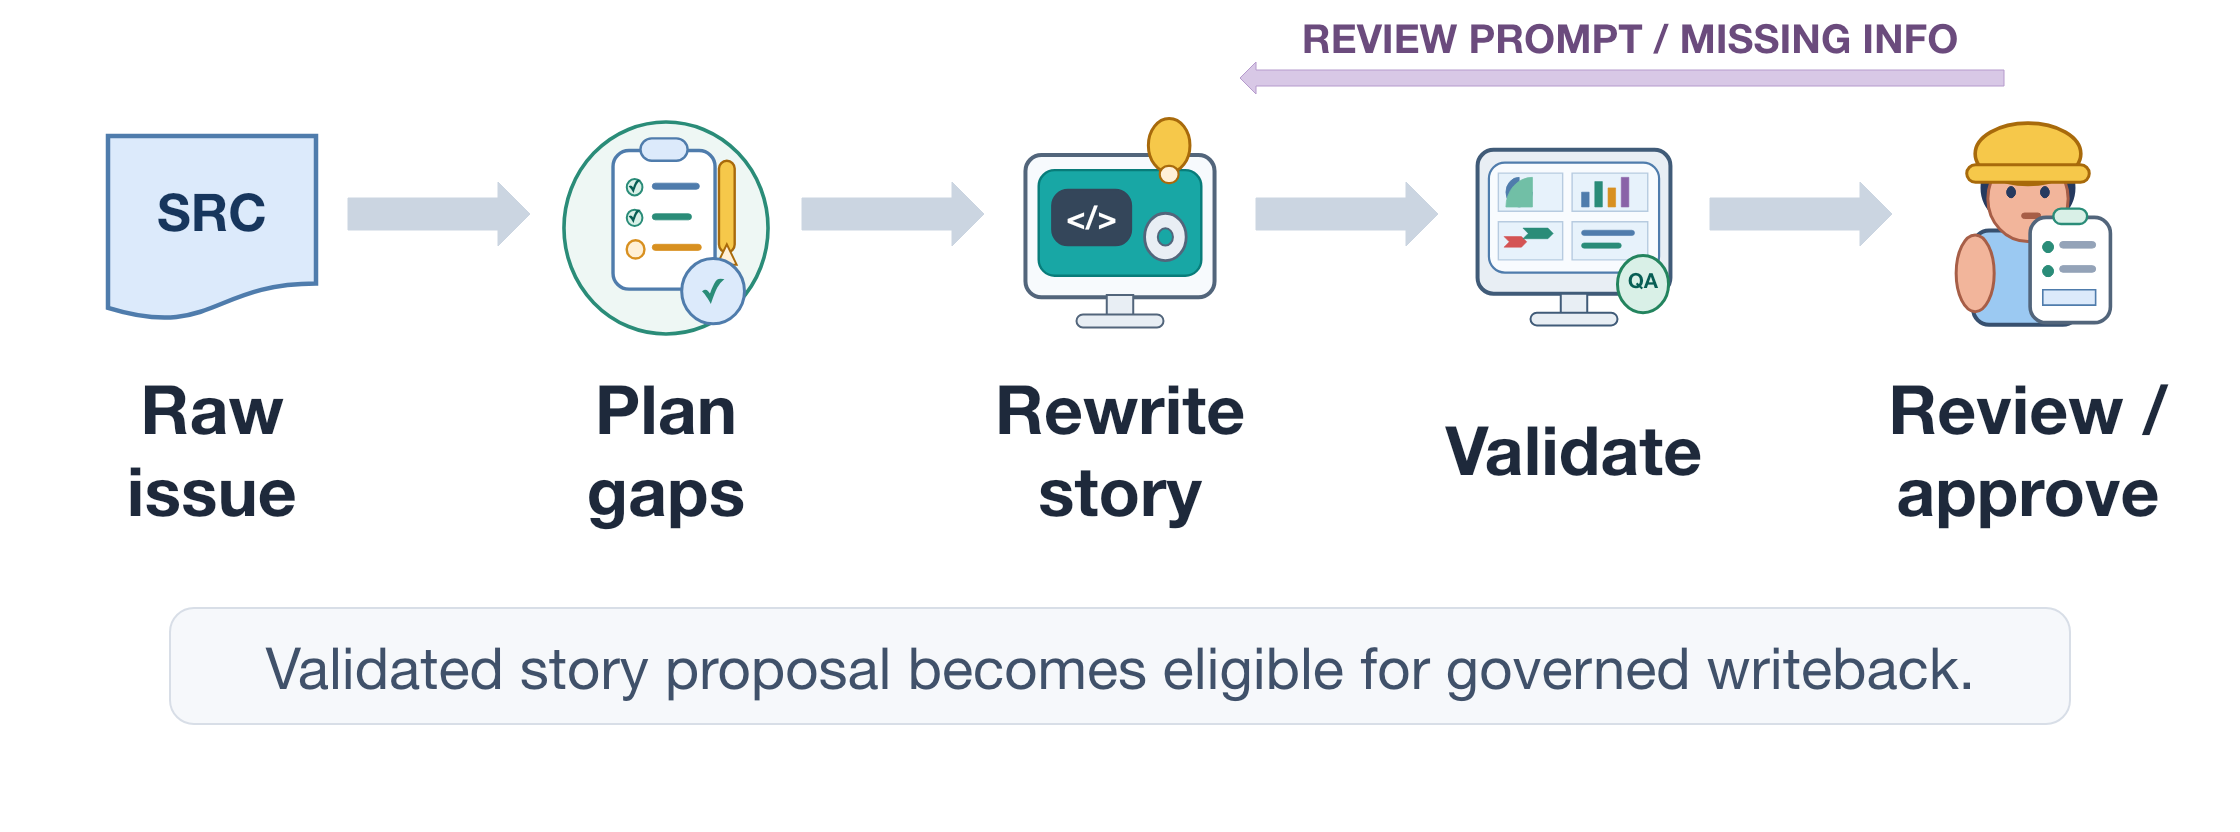
\includegraphics[width=\linewidth]{fig_agentic_module_story_issue_enhancer.png}
\caption{Agent module 1: improving stories and issues.}
\label{fig:module-story-issue}
\end{subfigure}
\par\medskip
\begin{subfigure}[t]{0.93\textwidth}
\centering
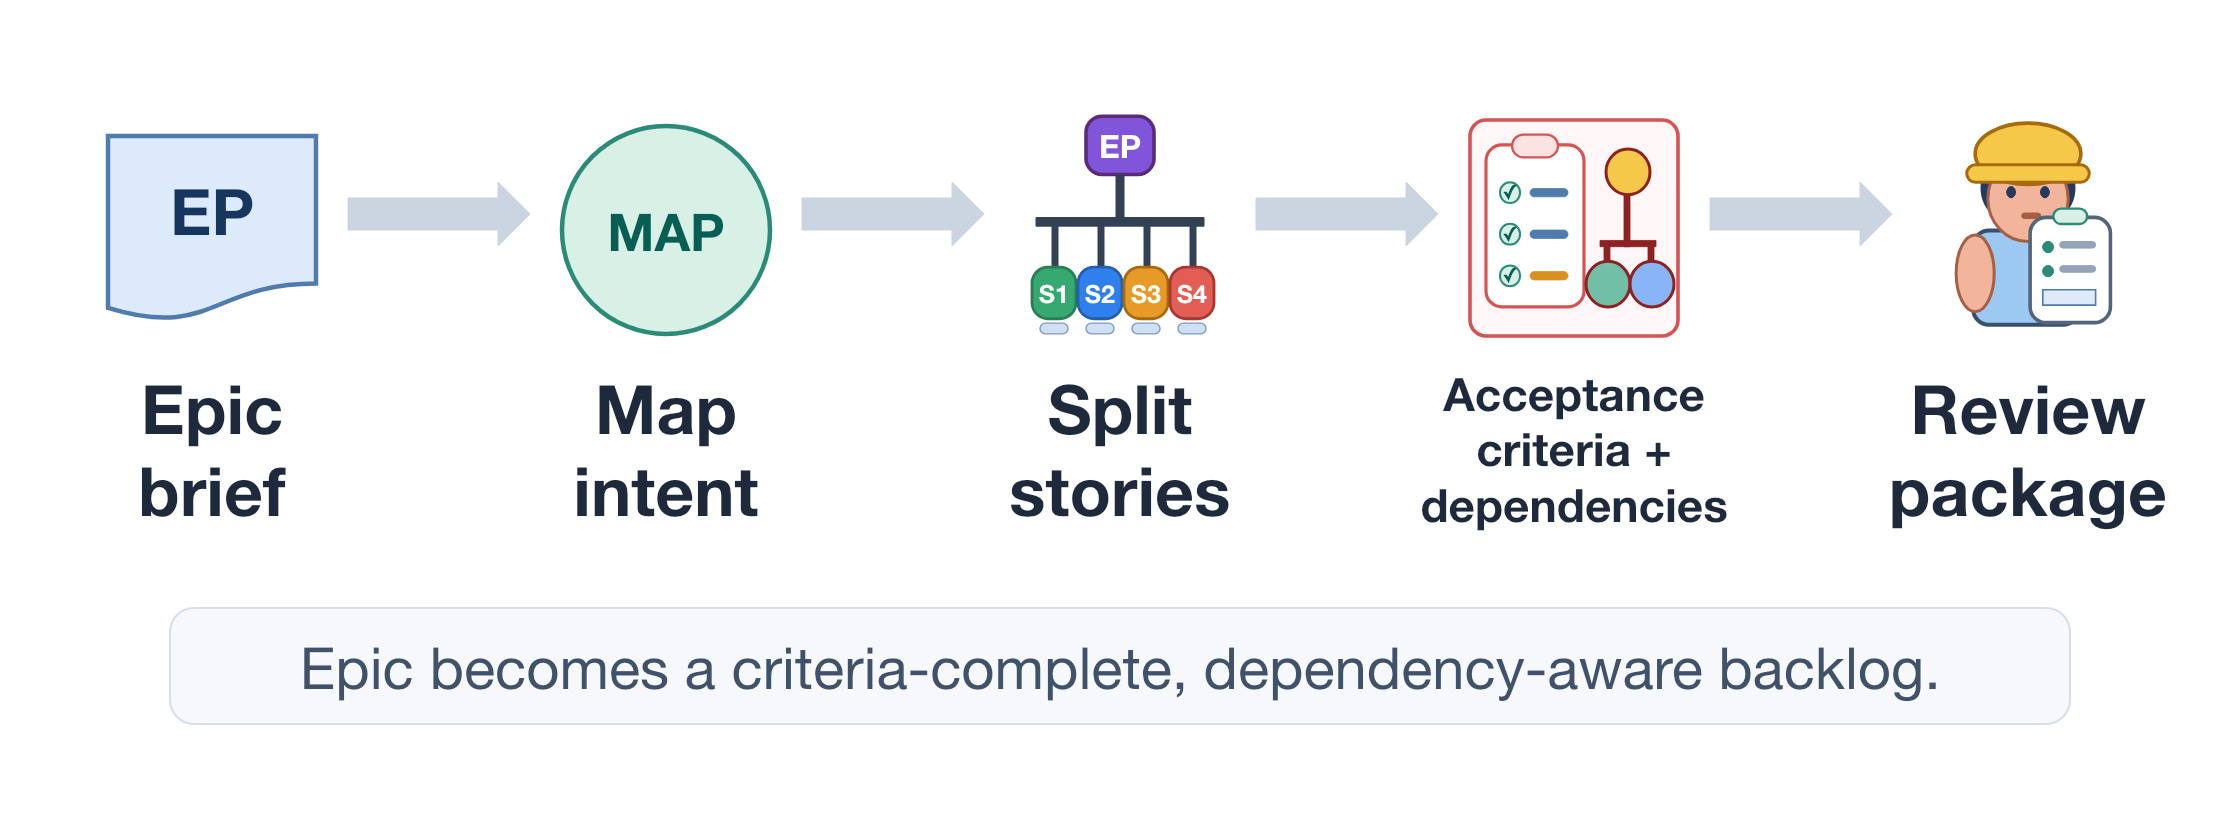
\includegraphics[width=\linewidth]{fig_agentic_module_epic_breaker.png}
\caption{Agent module 2: splitting epics into stories.}
\label{fig:module-epic-breaker}
\end{subfigure}

\caption{The four agent modules: improving stories and issues, splitting epics into stories, creating prompts, and selecting prompts through RL. These panels show the separate responsibilities within the overall system. Panels (c) and (d) continue on the next figure page.}
\label{fig:agentic-module-architecture}
\end{figure*}

\begin{figure*}[p]
\ContinuedFloat
\centering

\begin{subfigure}[t]{0.93\textwidth}
\centering
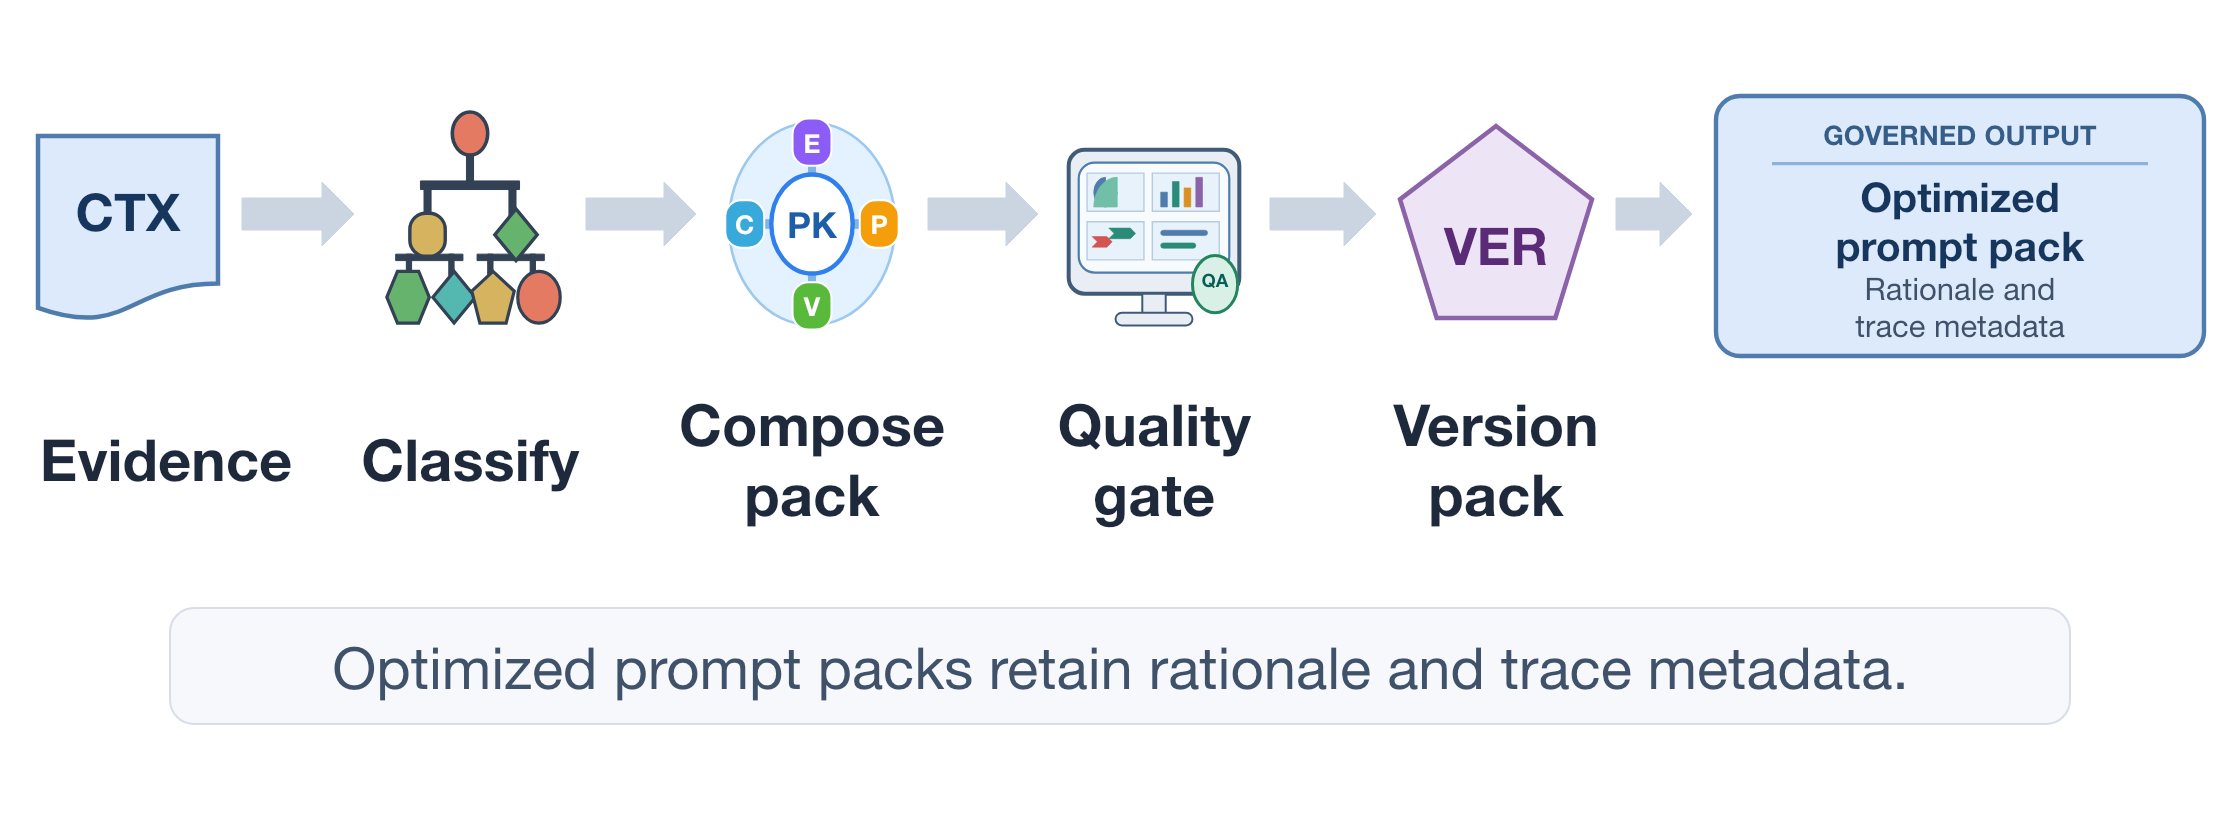
\includegraphics[width=\linewidth]{fig_agentic_module_prompt_generator.png}
\caption{Agent module 3: creating prompts.}
\label{fig:module-prompt-generator}
\end{subfigure}
\par\medskip
\begin{subfigure}[t]{0.93\textwidth}
\centering
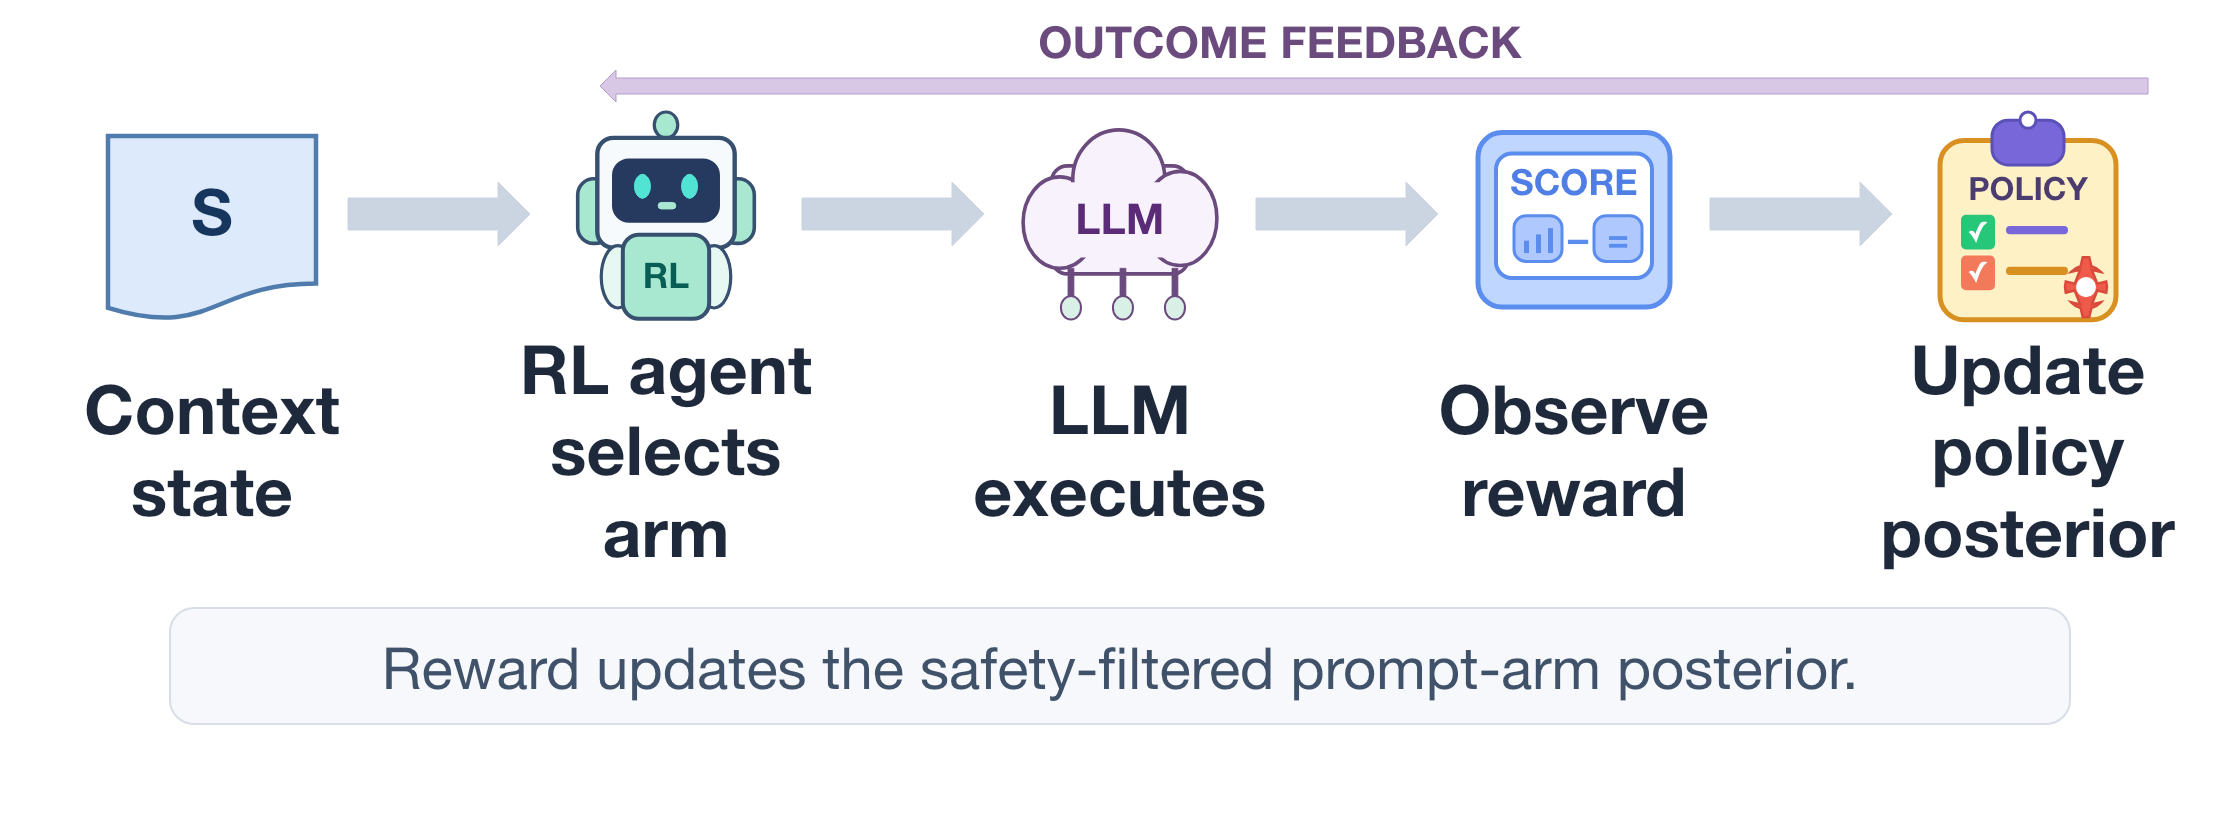
\includegraphics[width=\linewidth]{fig_agentic_module_rl_controller.png}
\caption{Agent module 4: RL controller.}
\label{fig:module-rl-controller}
\end{subfigure}
\caption{Agent modules (continued): creating prompts and selecting prompts through RL.}
\Description{Four-panel figure showing modules for improving stories and issues, splitting epics into stories, creating prompts, and selecting prompts through reinforcement learning.}

\end{figure*}
\FloatBarrier
% END preserved module_architecture.tex body

\FloatBarrier
\section{Records that explain each decision}
Each run records what it covers, who requested it, its time stamps, and the information used to prevent repeated writes. For each item, it also records the current state, confidence and readiness scores, policy flags, draft fields, evidence links, approval decisions and notes, and hashes before and after writeback. Keeping these records allows researchers to trace a planning decision for evaluation~\citep{R70,R54}, audit~\citep{R93}, or investigation of a problem.

The event history is not overwritten, so earlier events remain in order. A separate record of the current state can be updated for fast searches. Informational warnings describe small gaps. Advisory warnings draw the reviewer's attention to a problem. Blocking warnings prevent changes to Jira until the problem is fixed.

\FloatBarrier
\section{How an epic is split into stories}

\subsection{Drafting candidate stories}
The system uses the epic description and existing stories to identify work that is still needed. It can propose stories for:
\begin{itemize}
  \item the user interface and user interactions,
  \item APIs and the rules for exchanging data,
  \item storing data and writing approved changes,
  \item checking results and testing whether changes break existing behavior.
\end{itemize}

It compares both the words and the meaning of existing summaries. It skips types of stories whose work is already covered. This helps avoid creating tickets that describe the same work in different words.

The system also treats design information written directly in an epic as evidence. This can include design headings, scaling plans, formulas, APIs, workflows, checks, rollback plans, and tests. It records this evidence as \texttt{jira\_embedded\_context}. When a linked Confluence page is unavailable, the system can still plan within the information supplied by the epic itself. If the epic contains only links and those links cannot be opened, it reports that the needed context is unavailable and does not create placeholder stories.

\subsection{Assigning story points}
Story points are rough estimates of the work involved in a story. The starting estimate uses assumptions about its complexity:
\begin{equation}
\mathrm{SP}(s) = f(\xi_{\text{scope}}, \xi_{\text{integration}}, \xi_{\text{risk}}, \xi_{\text{unknown}}),
\end{equation}
The four $\xi$ terms are starting estimates for scope, connections to other systems, risk, and uncertainty, expressed on a common scale. The size categories are 3, 5, and 8 story points. The current implementation uses fixed defaults (3/5); learning these estimates from past work is left for future versions.

Fixed defaults give consistent starting estimates. They avoid changes caused by a learned estimation method before enough past data are available. They provide a consistent baseline for evaluating automation before other estimation methods are introduced.

\subsection{Reviewing and improving each draft}
For each candidate story $s$:
\begin{enumerate}
  \item check the meaning of the story,
  \item calculate its readiness and confidence scores,
  \item if $C(s)<\tau_c$, provide guidance and revise the story, up to the allowed number of attempts,
  \item return the story in the required data format.
\end{enumerate}
Here, $C(s)$ is the story's confidence score and $\tau_c$ is the required threshold. Reviewers can guide each revision by pointing out missed cases, unresolved dependencies, or unclear requirements about how the system should operate. These exchanges make revision a joint process between the reviewer and the AI \citep{R56,R57}.

In one version of the design, every draft follows the same set of fields, with a defined data type for each:
\texttt{problem\_statement}, \texttt{actor\_value}, \texttt{functional\_scope}, \texttt{nfr\_constraints}, \texttt{acceptance\_criteria},
\texttt{dependency\_map}, \texttt{risk\_register}, and \texttt{test\_considerations}. These fields describe the problem, the user's benefit, the planned functions, operating constraints, conditions for acceptance, dependencies, risks, and tests. A shared format helps review, analysis, and policy-checking tools read the same information without having to interpret free-form text.

The system can also use a coverage table to check the epic as a whole. Each column is a proposed story. The rows cover the user interface, APIs, data, understanding system behavior, handling and recovering from failures, and security. Gaps in this table identify areas that need more work, so the system can propose stories for those areas.

\subsection{Steps for comparing the methods}
Algorithm~\ref{alg:ablation-exec} describes which components are used for each of the four method definitions. This is called an ablation comparison: components can be left out to define a simpler method. The steps use a shared scorecard with fields for quality, efficiency, governance, the combined score, and assessment time. B0 requires an independently prepared manual package. The other modes run the template method, the one-shot language model, or the complete Jira Enhancer workflow. Each result keeps its status as a measured result or a result of the scoring analysis.

In the algorithm, the critic loop checks drafts and suggests revisions. The context packer selects and arranges source information. A validator checks the required fields and conditions. Governed writeback saves approved changes only after the workflow checks pass.

\begin{algorithm*}[H]
\DontPrintSemicolon
\footnotesize
\caption{Ablation-Mode Execution for B0/B1/B2/B3 Comparison}
\label{alg:ablation-exec}
\KwIn{Epic unit $E_u$, mode $m \in \{\mathrm{B0},\mathrm{B1},\mathrm{B2},\mathrm{B3}\}$}
\KwOut{Metric row $(Q_m,\mathrm{Eff}_m,G_m,\mathrm{Composite}_m,\mathrm{Time}_m)$}
\tcp{Apply the selected mode's component schema.}
\eIf{$m=\mathrm{B0}$}{
  ExecuteManualReferenceCore$(E_u)$\; \tcp*[r]{Independent manual package required}
}{
  ExecuteTemplateCore$(E_u)$ if $m=\mathrm{B1}$\;
  ExecuteGenericLLMCore$(E_u)$ if $m=\mathrm{B2}$\;
  ExecuteFullJiraEnhancerCore$(E_u)$ if $m=\mathrm{B3}$\;
}
\tcp{Disable B3-only components in baseline modes.}
\If{$m\neq\mathrm{B3}$}{
  Disable components excluded from mode $m$ (critic loop / context packer / validator / governed writeback)\;
}
\tcp{Use one scorer; each row retains its measured or analytical status.}
Collect metrics using the same scorer and schema across all modes\;
Compute $Q_m$ (quality), $\mathrm{Eff}_m$ (efficiency), $G_m$ (governance), $\mathrm{Composite}_m$, and $\mathrm{Time}_m$\;
\Return{$(Q_m,\mathrm{Eff}_m,G_m,\mathrm{Composite}_m,\mathrm{Time}_m)$}\;
\end{algorithm*}


\FloatBarrier

\clearpage
\appendix
\setcounter{table}{5}
\renewcommand{\thetable}{\thesection.\arabic{table}}
\section{Checking the Scoring Formulas with Repeatable Input Changes}\label{sec:stress-testing}
Table~\ref{tab:scoring-sanity-checks} shows scores calculated from formulas for two checks. The internal check reuses inputs derived from earlier system runs and changes them in repeatable ways using fixed random seeds (seeded perturbations). The public-input check applies the same formulas to 300 SWE-bench Lite issue texts~\citep{R26}. B0--B3 are scoring profiles in this table. Their composite, or combined score, is a weighted mean: quality, efficiency, and governance contribute weights of 0.45, 0.30, and 0.25, respectively, on a 0--100 scale. The weights determine how much each component contributes to the combined score. These rows check how the scoring formulas are implemented. They are separate from the results of running the baseline methods in Section~5.3 of the main manuscript.

\begin{table*}[htbp]
\centering
\setlength{\tabcolsep}{3pt}
\small
\caption{Checks of the scoring formulas using repeatable input changes. The reported scores are means calculated from formulas.}
\label{tab:scoring-sanity-checks}
\begin{tabular}{@{}llrrrrr@{}}
\toprule
Input & Scoring profile & Rows & Quality & Efficiency & Governance & Combined score \\
\midrule
Seeded internal units & B0 & 5,000 & 60.17 & 30.28 & 35.18 & 44.96 \\
 & B1 & 5,000 & 59.66 & 47.01 & 36.45 & 50.06 \\
 & B2 & 5,000 & 73.76 & 52.33 & 41.97 & 59.38 \\
 & B3 & 5,000 & 88.18 & 66.97 & 68.76 & 76.96 \\
\midrule
Public issue text & B0 & 300 & 60.39 & 30.62 & 35.21 & 45.16 \\
 & B1 & 300 & 57.72 & 48.20 & 35.34 & 49.27 \\
 & B2 & 300 & 79.36 & 48.39 & 42.79 & 60.93 \\
 & B3 & 300 & 89.92 & 66.65 & 69.72 & 77.89 \\
\bottomrule
\end{tabular}
\end{table*}




\clearpage
\section{Checking Whether Equal Weights Change the Comparison}\label{sec:weight-sensitivity}
We tested one fixed alternative to the priority weights: give all seven requirement dimensions equal weight. These uniform weights produce the arithmetic mean, or ordinary average: add the seven ratings and divide by seven. Each weight is exactly $1/7$ (approximately 14.286\%). The analysis uses the same corrected ratings from all 40 reviewers. It excludes the 160 masked-repeat ratings, which came from repeat assessments that were not marked as repeats. It averages the 1,680 primary ratings separately for each combination of epic and method. The 14 matched epics remain the units of inference: each epic is one case in the statistical comparison, with the methods compared on that same epic. We did not search for other weights or run an additional generation experiment.

For each B3--baseline comparison, we used an exact two-sided paired sign-flip test. It checks all $2^{14}$ ways of assigning signs to the paired epic differences to assess evidence for a difference in either direction. We also used 100,000 paired epic-bootstrap resamples to obtain percentile confidence intervals. This procedure draws whole epics with replacement, so an epic can appear more than once in a resample. It repeats the calculation while keeping the methods for each epic together. The intervals describe uncertainty in the estimated difference. The bootstrap seeds were 20261313 for B3--B2 and 20261314 for B3--B1, with identical resampling under both weight schemes. Holm adjustment reduces the risk of false-positive conclusions when several comparisons are tested. In the reported results, it covers the two contrasts within each weighting scheme. As an additional check for multiple testing, treating all four weighting--contrast tests as one family gives $p_{\mathrm{Holm}}=0.000488$ for every contrast.

\begin{table*}[htbp]
\centering
\footnotesize
\setlength{\tabcolsep}{3pt}
\caption{Comparison of requirement-quality scores under the two weighting schemes. Scores retain the 1--5 scale. Confidence intervals are calculated by resampling 14 matched epics; the reported Holm adjustment covers the two contrasts within each weighting scheme.}
\label{tab:weight-sensitivity}
\begin{tabularx}{\textwidth}{@{}ll>{\centering\arraybackslash}Xrr@{}}
\toprule
Weights & Comparison & Mean difference [95\% CI] & Holm $p$ & Epics favoring B3 \\
\midrule
Priority & B3--B2 & 0.542 [0.509, 0.573] & 0.000244 & 14/14 \\
Priority & B3--B1 & 1.592 [1.205, 1.984] & 0.000244 & 14/14 \\
Uniform & B3--B2 & 0.559 [0.547, 0.571] & 0.000244 & 14/14 \\
Uniform & B3--B1 & 1.547 [1.210, 1.873] & 0.000244 & 14/14 \\
\bottomrule
\end{tabularx}
\end{table*}

The mean scores under uniform weights are 2.737, 3.724, and 4.283 for B1, B2, and B3, respectively. Table~\ref{tab:weight-sensitivity} shows that B3 scores higher than each baseline on every epic under both tested weighting schemes. The direction of the comparison in this corrected dataset therefore does not depend on using the selected priority weights. This repeat analysis does not independently check whether the rating corrections are accurate or show that the results remain stable on new portfolios.


\FloatBarrier

\clearpage
\subsection*{Radar Plot of Reviewer Ratings}
\phantomsection
\addcontentsline{toc}{subsection}{Radar Plot of Reviewer Ratings}
\begin{figure}[H]
\centering
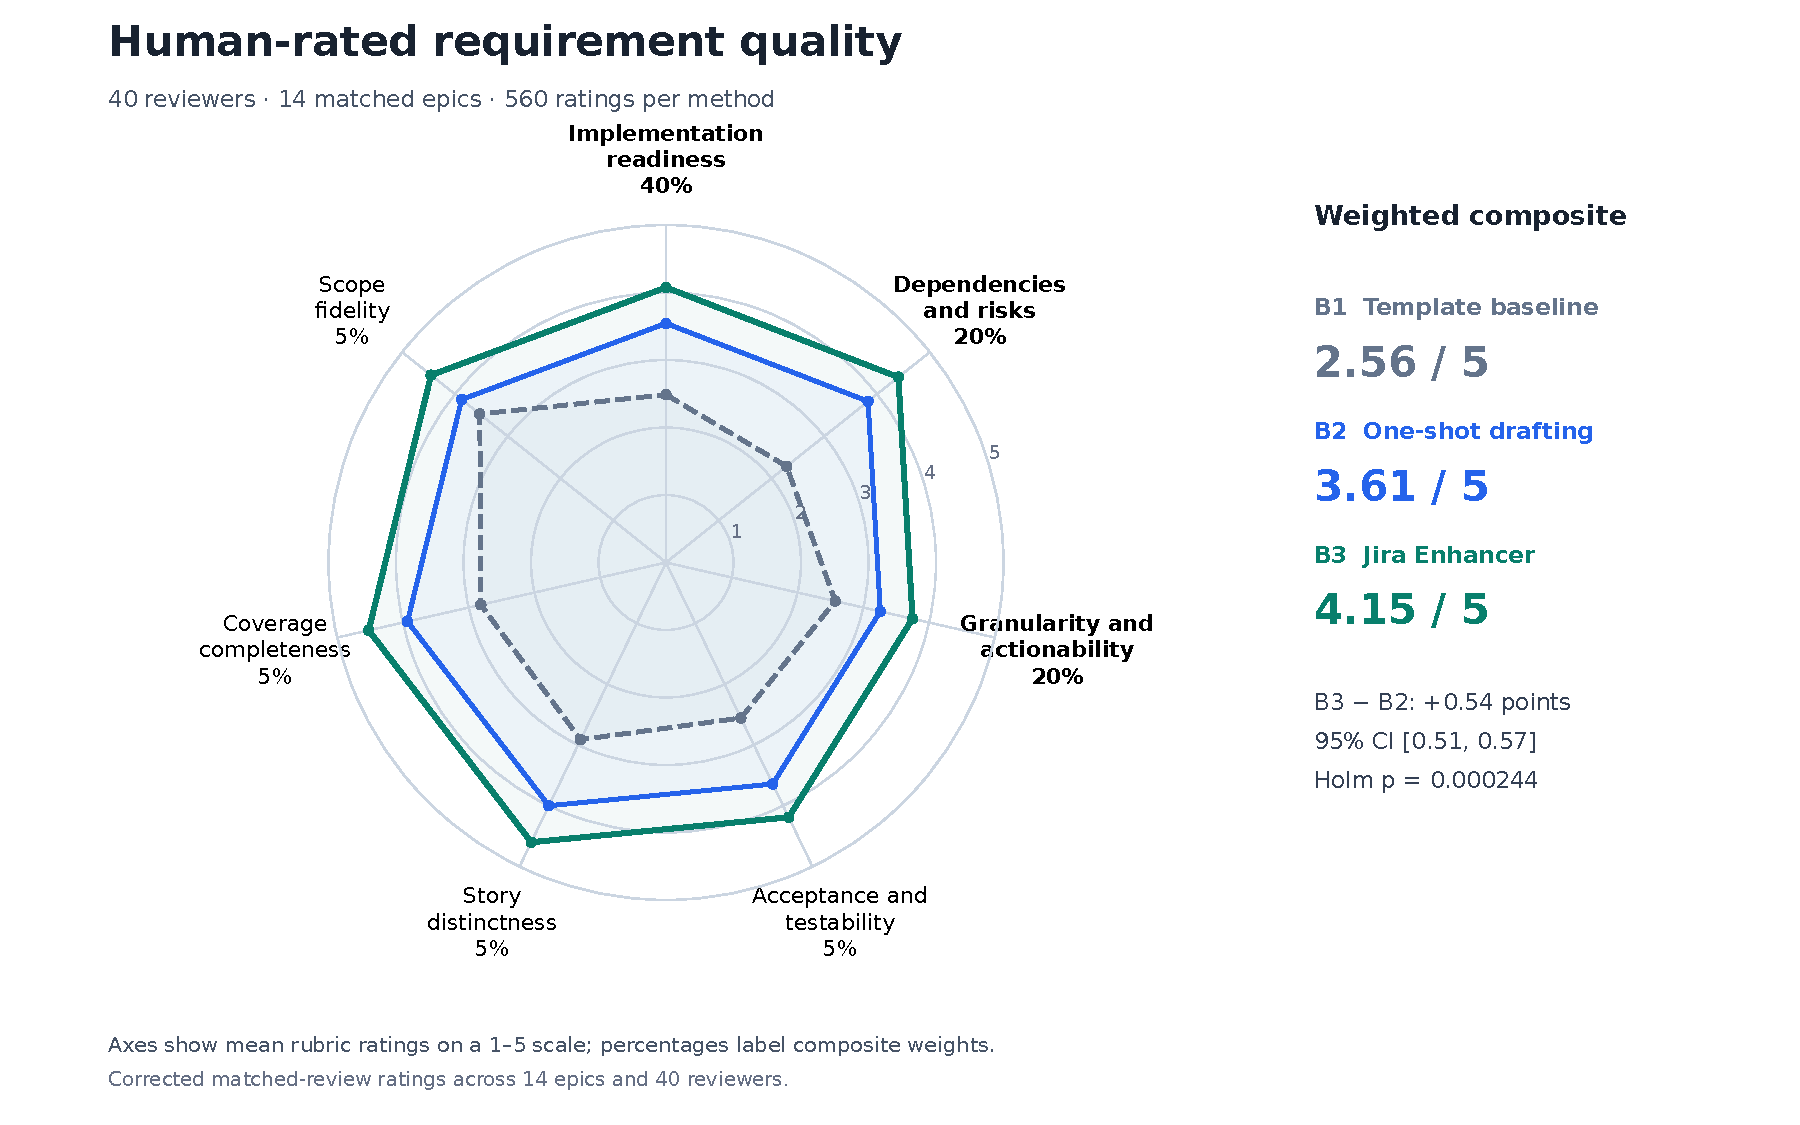
\includegraphics[width=\linewidth]{../patent/reviewer_study/public_results/matched_review_weighted_radar.pdf}
\caption{Reviewer ratings of requirement quality for B1 (template baseline), B2 (one-shot drafting), and B3 (Jira Enhancer). Each spoke of the radar plot shows the mean rating for a requirement dimension on the anchored 1--5 scale, whose scores have defined descriptions. There are seven dimensions. The percentages beside the axes give the weights used to calculate the priority composite, or combined score, on the right. The plotted points show the dimension means before weighting.}
\label{fig:supp-matched-review-radar}
\end{figure}

\paragraph{Data shown in the figure.}
The figure uses the corrected matched-review data from 40 reviewers and 14 epic packages per method, giving 560 primary package ratings for each method. The 160 masked-repeat ratings are excluded. B3 uses RL-guided prompt selection and refines drafts within a set limit on attempts. It has higher mean ratings on all seven dimensions. Implementation readiness receives 40\% of the composite weight; dependencies and risks and granularity and actionability receive 20\% each; the other four dimensions receive 5\% each.

The priority-weighted mean scores are 2.56 for B1, 3.61 for B2, and 4.15 for B3. The B3--B2 paired difference is +0.54 points, with a 95\% epic-bootstrap confidence interval of [0.51, 0.57] and Holm-adjusted exact paired sign-flip $p=0.000244$. The 14 matched epics are the cases used for statistical inference, and the Holm adjustment covers the two declared baseline contrasts. These are the same results reported in Section 5.3 of the main manuscript. The equal-weight comparison is also reported there and in Supplementary Appendix~\ref{sec:weight-sensitivity}.

\paragraph{Data and how to reproduce the plot.}
The original graphic is unchanged. It uses the public \href{https://github.com/anonymous94u/JiraEnhancer/blob/main/patent/reviewer_study/public_results/matched_review_quality_factor_comparison.csv}{dimension means and weights}, \href{https://github.com/anonymous94u/JiraEnhancer/blob/main/patent/reviewer_study/public_results/matched_review_method_summary.csv}{method summaries}, and \href{https://github.com/anonymous94u/JiraEnhancer/blob/main/patent/reviewer_study/public_results/matched_review_pairwise.csv}{paired comparisons}. The \href{https://github.com/anonymous94u/JiraEnhancer/blob/main/patent/reviewer_study/plot_weighted_review_radar.py}{plotting script} and \href{https://github.com/anonymous94u/JiraEnhancer/blob/main/patent/reviewer_study/public_results/matched_review_weighted_radar.pdf}{original vector PDF} are available in the same repository.

\FloatBarrier
\clearpage
\section{Update Test Results by Scenario}\label{sec:fault-scenario-matrix}
Table~\ref{tab:fault-scenario-matrix} gives the results for each test scenario behind Table~5b of the main manuscript. A transaction is one intended update to Jira, including any retry attempts. Each scenario has 2,000 observations for each configuration. Random seed 20260726 sets the shuffled order of 18,000 transactions. All configurations use this same order, giving 72,000 observations in total. The valid-control scenario and two retry scenarios provide 6,000 transactions that are eligible for an update in each configuration. The other six scenarios provide 12,000 transactions where the reviewed state has changed.

A stale update uses approval for an earlier state that is no longer valid. In the source ABA scenario, the source changes and then returns to the same text. A content hash, or digital fingerprint, can miss this change because the final text is unchanged. Draft, policy, and target drift mean that the draft, rules, or update destination changed after review. A response-loss retry repeats a request after the caller does not receive confirmation of the first attempt.

\begin{table*}[htbp]
\centering
\footnotesize
\setlength{\tabcolsep}{3pt}
\caption{Results for every update test scenario. Each cell reports $(m,s,d)$: the mean number of modeled updates per transaction, whether an update used stale approval, and whether an update was repeated. The last two entries are 0 or 1 because their rates are 0\% or 100\% in every cell.}
\label{tab:fault-scenario-matrix}
\begin{tabularx}{\textwidth}{@{}>{\raggedright\arraybackslash}X*{4}{>{\centering\arraybackslash}p{0.13\textwidth}}@{}}
\toprule
Scenario & A0 & A1 & A2 & A3 \\
\midrule
Valid control & $(1,0,0)$ & $(1,0,0)$ & $(1,0,0)$ & $(1,0,0)$ \\
Source edit & $(1,1,0)$ & $(0,0,0)$ & $(0,0,0)$ & $(0,0,0)$ \\
Source ABA & $(1,1,0)$ & $(1,1,0)$ & $(1,1,0)$ & $(0,0,0)$ \\
Draft drift & $(1,1,0)$ & $(1,1,0)$ & $(1,1,0)$ & $(0,0,0)$ \\
Policy drift & $(1,1,0)$ & $(1,1,0)$ & $(1,1,0)$ & $(0,0,0)$ \\
Target drift & $(1,1,0)$ & $(1,1,0)$ & $(1,1,0)$ & $(0,0,0)$ \\
Response-loss retry & $(2,0,1)$ & $(2,0,1)$ & $(1,0,0)$ & $(1,0,0)$ \\
Concurrent retry (modeled) & $(2,0,1)$ & $(2,0,1)$ & $(1,0,0)$ & $(1,0,0)$ \\
Combined source/draft drift & $(2,1,1)$ & $(0,0,0)$ & $(0,0,0)$ & $(0,0,0)$ \\
\bottomrule
\end{tabularx}
\end{table*}

A0 uses ordinary approval and a log. A1 also checks the source hash. A2 adds atomic idempotency, which prevents repeated requests from repeating the update. A3 adds a transaction envelope, a record that links approval to the reviewed source version, draft, rules, and allowed update targets.

The test program calls the implemented A3 envelope builder and validator. It counts modeled updates as zero for a blocked transaction, one for an allowed A2/A3 transaction, and the number of attempts for an allowed A0/A1 transaction. These are modeled counts based on the validation results and the stated update rules. They are not observations of actual remote Jira updates.

The concurrent-retry scenario contains two attempts. The program does not send parallel network requests. Seven separate workflow tests use a mock connector, which stands in for the remote service. They include retries after completed updates and recovery when a commit response is lost. These tests do not measure how often failures occur in production or how the system performs under concurrent load.

% Insertion draft: place after Appendix C and before backmatter/bibliography.
% No issue keys, internal URLs, pod names, or subscription identifiers are included.
\section{Implementation Case: Moving Subscriptions Between Service Instances}\label{sec:downstream-rebalancing-case}

\subsection{Case origin and subscription placement}
The author identifies this enhancement as work derived from Jira Enhancer. It spans three implementation stories: the subscriber service, Java SDK, and Python SDK. An SDK is a software development kit that client programs use to work with the service. The run records below cover the subscriber service and Python SDK. The companion story-case manifest lists the components and their supporting records. The Jira Enhancer origin is the author's attribution; the run records do not independently establish that origin.

The saved run archives contain tests from 15 October 2026 in a development cloud environment. One run had the pooling option enabled and the other had it disabled. An independent check recalculated all 19 listed file hashes in each archive. It also inspected the recorded observations, snapshots after each stage, and records of transfers between service instances. This check verified saved files and records; it did not rerun the tests.

Each run kept five Python client programs active, with 100, 200, 500, 1,000, and 1,500 subscriptions, respectively. A subscription requests events from the service. A client--subscription binding links a client to a subscription. The runs had 3,300 such bindings across 1,500 distinct logical subscription identifiers; different clients could use the same subscription identifier.

A pod is a running instance of the service. The pod count was increased manually from one to two, three, and four. At each observed stage after increasing the pod count, the clients remained active for at least the required 420-second hold. Table~\ref{tab:downstream-binding-distribution} shows the ready bindings at the end of each stage. Pod labels follow creation order within each run and do not identify the same pod across runs.

\begin{table*}[htbp]
\centering
\footnotesize
\setlength{\tabcolsep}{3pt}
\caption{Ready client--subscription bindings after each manual increase in pod count. Hold is the shortest time a client remained active in that stage. Each row totals 3,300 bindings; a dash means that the pod had not yet been created. The required minimum hold was 420 seconds.}
\label{tab:downstream-binding-distribution}
\begin{tabular}{@{}lrrrrrr@{}}
\toprule
Pooling & Pods & P1 & P2 & P3 & P4 & Hold (s) \\
\midrule
Enabled & 2 & 1,860 & 1,440 & -- & -- & 456.9 \\
Enabled & 3 & 1,240 & 1,150 & 910 & -- & 444.8 \\
Enabled & 4 & 930 & 840 & 810 & 720 & 442.3 \\
\addlinespace
Disabled & 2 & 1,700 & 1,600 & -- & -- & 443.2 \\
Disabled & 3 & 800 & 1,500 & 1,000 & -- & 433.3 \\
Disabled & 4 & 500 & 1,500 & 1,000 & 300 & 439.3 \\
\bottomrule
\end{tabular}
\end{table*}

\subsection{Transfer records, status messages, and findings}
A handoff transfers responsibility for subscriptions from one service instance to another. Table~\ref{tab:downstream-handoff-telemetry} summarizes these transfers and the status messages recorded during the runs. Completed handoffs recorded these phases: \texttt{handshake}, \texttt{promote}, \texttt{ready}, \texttt{commit}, \texttt{quiesce}, \texttt{drain}, \texttt{retire\_\allowbreak{}authorized}, and \texttt{retire}. These are the phase names used in the logs.

The checks linked the recorded transfer of ownership to subscription receipts from the same session and to \texttt{DRAINED} and \texttt{RETIRED} responses from the original service instance. The enabled archive contains 14 complete sequences (112 phase records). The disabled archive contains six (48 records). No additional incomplete sequence was found in the inspected handoff records. Five handoffs in the disabled run moved bindings to newly created pods. They account for 2,900 of that run's 3,000 binding moves. These totals count each transfer, so a binding moved more than once contributes more than once.

\begin{table*}[htbp]
\centering
\small
\caption{Transfer records and MainStats status messages from the saved runs. Probe messages are excluded. Time intervals are measured between successive messages from the same client, physical connection, and session.}
\label{tab:downstream-handoff-telemetry}
\begin{tabularx}{\textwidth}{@{}Xrr@{}}
\toprule
Recorded quantity & Enabled & Disabled \\
\midrule
Complete handoffs / phase records & 14 / 112 & 6 / 48 \\
Cumulative binding moves & 3,070 & 3,000 \\
MainStats messages, excluding probes & 2,476 & 933 \\
Connection--session groups & 27 & 11 \\
Message intervals within each group & 2,449 & 922 \\
Median interval (seconds) & 10.000391 & 10.000380 \\
Maximum interval (seconds) & 10.205 & 10.208 \\
Intervals above 11 seconds & 0 & 0 \\
Business events / ACKs / NACKs & 0 / 0 / 0 & 0 / 0 / 0 \\
\bottomrule
\end{tabularx}
\end{table*}

All five Python workers exited with status zero, indicating successful completion, in each run. The records verify subscription placement and handoffs that require subscription receipts before proceeding. MainStats is the name of the recorded status messages. The intervals show how regularly those messages arrived. ACKs confirm successful handling of a message; NACKs report a failure to handle it. No business events, ACKs, or NACKs were recorded, so these runs do not test business-event delivery.

The saved snapshots, completed handoff sequences, and successful worker exits show that this rebalancing enhancement could run in the tested development setting. The records cover subscription placement and transfer, not production reliability or a comparison of planning methods.

\FloatBarrier

\clearpage
\phantomsection
\addcontentsline{toc}{section}{References}
\begin{thebibliography}{25}

\bibitem[{Lucassen et~al.(2016)Lucassen, Dalpiaz, van~der Werf, and
  Brinkkemper}]{R52}
\bibinfo{author}{G.~Lucassen}, \bibinfo{author}{F.~Dalpiaz},
  \bibinfo{author}{J.~M. E.~M. van~der Werf}, \bibinfo{author}{S.~Brinkkemper},
\newblock \bibinfo{title}{Improving agile requirements: The quality user story
  framework and tool},
\newblock \bibinfo{journal}{Requirements Engineering} \bibinfo{volume}{21}
  (\bibinfo{year}{2016}) \bibinfo{pages}{383--403}.
%Type = Article
\bibitem[{{ISO/IEC/IEEE}(2018)}]{R62}
\bibinfo{author}{{ISO/IEC/IEEE}}, \bibinfo{title}{ISO/IEC/IEEE 29148:2018
  Systems and Software Engineering---Life Cycle Processes---Requirements
  Engineering}, \bibinfo{organization}{ISO/IEC/IEEE}, \bibinfo{year}{2018}.
%Type = Inproceedings
\bibitem[{Cao and Ramesh(2008)}]{R63}
\bibinfo{author}{L.~Cao}, \bibinfo{author}{B.~Ramesh},
\newblock \bibinfo{title}{Agile requirements engineering practices: An
  empirical study},
\newblock \bibinfo{journal}{IEEE Software} \bibinfo{volume}{25}
  (\bibinfo{year}{2008}) \bibinfo{pages}{60--67}.
%Type = Article
\bibitem[{Brown et~al.(2020)Brown, Mann, Ryder, Subbiah, Kaplan, Dhariwal,
  Neelakantan, Shyam, Sastry, Askell, Agarwal, Herbert-Voss, Krueger, Henighan,
  Child, Ramesh, Ziegler, Wu, Winter, Hesse, Chen, Sigler, Litwin, Gray, Chess,
  Clark, Berner, McCandlish, Radford, Sutskever, and Amodei}]{R1}
\bibinfo{author}{T.~B. Brown}, \bibinfo{author}{B.~Mann},
  \bibinfo{author}{N.~Ryder}, \bibinfo{author}{M.~Subbiah},
  \bibinfo{author}{J.~Kaplan}, \bibinfo{author}{P.~Dhariwal},
  \bibinfo{author}{A.~Neelakantan}, \bibinfo{author}{P.~Shyam},
  \bibinfo{author}{G.~Sastry}, \bibinfo{author}{A.~Askell},
  \bibinfo{author}{S.~Agarwal}, \bibinfo{author}{A.~Herbert-Voss},
  \bibinfo{author}{G.~Krueger}, \bibinfo{author}{T.~Henighan},
  \bibinfo{author}{R.~Child}, \bibinfo{author}{A.~Ramesh},
  \bibinfo{author}{D.~Ziegler}, \bibinfo{author}{J.~Wu},
  \bibinfo{author}{C.~Winter}, \bibinfo{author}{C.~Hesse},
  \bibinfo{author}{M.~Chen}, \bibinfo{author}{E.~Sigler},
  \bibinfo{author}{M.~Litwin}, \bibinfo{author}{S.~Gray},
  \bibinfo{author}{B.~Chess}, \bibinfo{author}{J.~Clark},
  \bibinfo{author}{C.~Berner}, \bibinfo{author}{S.~McCandlish},
  \bibinfo{author}{A.~Radford}, \bibinfo{author}{I.~Sutskever},
  \bibinfo{author}{D.~Amodei},
\newblock \bibinfo{title}{Language models are few-shot learners},
\newblock in: \bibinfo{booktitle}{Advances in Neural Information Processing
  Systems (NeurIPS)}, volume~\bibinfo{volume}{33}, \bibinfo{publisher}{Curran
  Associates, Inc.}, \bibinfo{address}{Red Hook, NY, USA},
  \bibinfo{year}{2020}, pp. \bibinfo{pages}{1877--1901}.
%Type = Inproceedings
\bibitem[{Wei et~al.(2022)Wei, Wang, Schuurmans, Bosma, Ichter, Xia, Chi, Le,
  and Zhou}]{R14}
\bibinfo{author}{J.~Wei}, \bibinfo{author}{X.~Wang},
  \bibinfo{author}{D.~Schuurmans}, \bibinfo{author}{M.~Bosma},
  \bibinfo{author}{B.~Ichter}, \bibinfo{author}{F.~Xia},
  \bibinfo{author}{E.~Chi}, \bibinfo{author}{Q.~V. Le},
  \bibinfo{author}{D.~Zhou},
\newblock \bibinfo{title}{Chain-of-thought prompting elicits reasoning in large
  language models},
\newblock in: \bibinfo{booktitle}{Advances in Neural Information Processing
  Systems (NeurIPS)}, volume~\bibinfo{volume}{35}, \bibinfo{publisher}{Curran
  Associates, Inc.}, \bibinfo{address}{Red Hook, NY, USA},
  \bibinfo{year}{2022}, pp. \bibinfo{pages}{24824--24837}.
  \DOIprefix\doi{10.52202/068431-1800}.
%Type = Inproceedings
\bibitem[{Fan et~al.(2023)Fan, Gokkaya, Harman, Lyubarskiy, Sengupta, Yoo, and
  Zhang}]{R59}
\bibinfo{author}{A.~Fan}, \bibinfo{author}{B.~Gokkaya},
  \bibinfo{author}{M.~Harman}, \bibinfo{author}{M.~Lyubarskiy},
  \bibinfo{author}{S.~Sengupta}, \bibinfo{author}{S.~Yoo},
  \bibinfo{author}{J.~M. Zhang},
\newblock \bibinfo{title}{Large language models for software engineering:
  Survey and open problems},
\newblock in: \bibinfo{booktitle}{2023 IEEE/ACM International Conference on
  Software Engineering: Future of Software Engineering (ICSE-FoSE)},
  \bibinfo{publisher}{IEEE}, \bibinfo{address}{Melbourne, Australia},
  \bibinfo{year}{2023}, pp. \bibinfo{pages}{31--53}.
  \DOIprefix\doi{10.1109/ICSE-FoSE59343.2023.00008}.
%Type = Inproceedings
\bibitem[{Barke et~al.(2023)Barke, James, and Polikarpova}]{R77}
\bibinfo{author}{S.~Barke}, \bibinfo{author}{M.~B. James},
  \bibinfo{author}{N.~Polikarpova},
\newblock \bibinfo{title}{Grounded copilot: How programmers interact with
  code-generating models},
\newblock \bibinfo{journal}{Proceedings of the ACM on Programming Languages}
  \bibinfo{volume}{7} (\bibinfo{year}{2023}) \bibinfo{pages}{85--111}.
%Type = Inproceedings
\bibitem[{Lewis et~al.(2020)Lewis, Perez, Piktus, Petroni, Karpukhin, Goyal,
  K{\"u}ttler, Lewis, Yih, Rockt{\"a}schel, Riedel, and Kiela}]{R3}
\bibinfo{author}{P.~Lewis}, \bibinfo{author}{E.~Perez},
  \bibinfo{author}{A.~Piktus}, \bibinfo{author}{F.~Petroni},
  \bibinfo{author}{V.~Karpukhin}, \bibinfo{author}{N.~Goyal},
  \bibinfo{author}{H.~K{\"u}ttler}, \bibinfo{author}{M.~Lewis},
  \bibinfo{author}{W.-t. Yih}, \bibinfo{author}{T.~Rockt{\"a}schel},
  \bibinfo{author}{S.~Riedel}, \bibinfo{author}{D.~Kiela},
\newblock \bibinfo{title}{Retrieval-augmented generation for
  knowledge-intensive nlp tasks},
\newblock in: \bibinfo{booktitle}{Advances in Neural Information Processing
  Systems (NeurIPS)}, volume~\bibinfo{volume}{33}, \bibinfo{publisher}{Curran
  Associates, Inc.}, \bibinfo{address}{Red Hook, NY, USA},
  \bibinfo{year}{2020}, pp. \bibinfo{pages}{9459--9474}.
%Type = Inproceedings
\bibitem[{Karpukhin et~al.(2020)Karpukhin, Oguz, Min, Lewis, Wu, Edunov, Chen,
  and Yih}]{R5}
\bibinfo{author}{V.~Karpukhin}, \bibinfo{author}{B.~Oguz},
  \bibinfo{author}{S.~Min}, \bibinfo{author}{P.~Lewis},
  \bibinfo{author}{L.~Wu}, \bibinfo{author}{S.~Edunov},
  \bibinfo{author}{D.~Chen}, \bibinfo{author}{W.-t. Yih},
\newblock \bibinfo{title}{Dense passage retrieval for open-domain question
  answering},
\newblock in: \bibinfo{booktitle}{Proceedings of the 2020 Conference on
  Empirical Methods in Natural Language Processing (EMNLP)},
  \bibinfo{publisher}{Association for Computational Linguistics},
  \bibinfo{address}{Online}, \bibinfo{year}{2020}, pp.
  \bibinfo{pages}{6769--6781}. \URLprefix
  \url{https://aclanthology.org/2020.emnlp-main.550/}.
  \DOIprefix\doi{10.18653/v1/2020.emnlp-main.550}.
%Type = Inproceedings
\bibitem[{Asai et~al.(2024)Asai, Min, Zhong, Chen, Hajishirzi, Yih, Choi,
  Lewis, and Zettlemoyer}]{R22}
\bibinfo{author}{A.~Asai}, \bibinfo{author}{S.~Min},
  \bibinfo{author}{Z.~Zhong}, \bibinfo{author}{D.~Chen},
  \bibinfo{author}{H.~Hajishirzi}, \bibinfo{author}{W.-t. Yih},
  \bibinfo{author}{Y.~Choi}, \bibinfo{author}{M.~Lewis},
  \bibinfo{author}{L.~Zettlemoyer},
\newblock \bibinfo{title}{Self-rag: Learning to retrieve, generate, and
  critique through self-reflection},
\newblock in: \bibinfo{booktitle}{International Conference on Learning
  Representations (ICLR)}, \bibinfo{publisher}{OpenReview.net},
  \bibinfo{address}{Vienna, Austria}, \bibinfo{year}{2024}.
%Type = Inproceedings
\bibitem[{Schick et~al.(2023)Schick, Dwivedi-Yu, Dess{\`i}, Raileanu, Lomeli,
  Hambro, Zettlemoyer, Cancedda, and Scialom}]{R17}
\bibinfo{author}{T.~Schick}, \bibinfo{author}{J.~Dwivedi-Yu},
  \bibinfo{author}{R.~Dess{\`i}}, \bibinfo{author}{R.~Raileanu},
  \bibinfo{author}{M.~Lomeli}, \bibinfo{author}{E.~Hambro},
  \bibinfo{author}{L.~Zettlemoyer}, \bibinfo{author}{N.~Cancedda},
  \bibinfo{author}{T.~Scialom},
\newblock \bibinfo{title}{Toolformer: Language models can teach themselves to
  use tools},
\newblock in: \bibinfo{booktitle}{Advances in Neural Information Processing
  Systems (NeurIPS)}, volume~\bibinfo{volume}{36}, \bibinfo{publisher}{Curran
  Associates, Inc.}, \bibinfo{address}{Red Hook, NY, USA},
  \bibinfo{year}{2023}, pp. \bibinfo{pages}{68539--68551}.
  \DOIprefix\doi{10.52202/075280-2997}.
%Type = Inproceedings
\bibitem[{Liu et~al.(2024)Liu, Yu, Zhang, Xu, Lei, Lai, Gu, Ding, Men, Yang,
  Zhang, Deng, Zeng, Du, Zhang, Shen, Zhang, Su, Sun, Huang, Dong, and
  Tang}]{R27}
\bibinfo{author}{X.~Liu}, \bibinfo{author}{H.~Yu}, \bibinfo{author}{H.~Zhang},
  \bibinfo{author}{Y.~Xu}, \bibinfo{author}{X.~Lei}, \bibinfo{author}{H.~Lai},
  \bibinfo{author}{Y.~Gu}, \bibinfo{author}{H.~Ding}, \bibinfo{author}{K.~Men},
  \bibinfo{author}{K.~Yang}, \bibinfo{author}{S.~Zhang},
  \bibinfo{author}{X.~Deng}, \bibinfo{author}{A.~Zeng},
  \bibinfo{author}{Z.~Du}, \bibinfo{author}{C.~Zhang},
  \bibinfo{author}{S.~Shen}, \bibinfo{author}{T.~Zhang},
  \bibinfo{author}{Y.~Su}, \bibinfo{author}{H.~Sun},
  \bibinfo{author}{M.~Huang}, \bibinfo{author}{Y.~Dong},
  \bibinfo{author}{J.~Tang},
\newblock \bibinfo{title}{Agentbench: Evaluating llms as agents},
\newblock in: \bibinfo{booktitle}{The Twelfth International Conference on
  Learning Representations}, \bibinfo{publisher}{OpenReview.net},
  \bibinfo{address}{Vienna, Austria}, \bibinfo{year}{2024}. \URLprefix
  \url{https://openreview.net/forum?id=zAdUB0aCTQ}.
%Type = Inproceedings
\bibitem[{Wu et~al.(2024)Wu, Bansal, Zhang, Wu, Li, Zhu, Jiang, Zhang, Zhang,
  Liu, Awadallah, White, Burger, and Wang}]{R28}
\bibinfo{author}{Q.~Wu}, \bibinfo{author}{G.~Bansal},
  \bibinfo{author}{J.~Zhang}, \bibinfo{author}{Y.~Wu}, \bibinfo{author}{B.~Li},
  \bibinfo{author}{E.~Zhu}, \bibinfo{author}{L.~Jiang},
  \bibinfo{author}{X.~Zhang}, \bibinfo{author}{S.~Zhang},
  \bibinfo{author}{J.~Liu}, \bibinfo{author}{A.~H. Awadallah},
  \bibinfo{author}{R.~W. White}, \bibinfo{author}{D.~Burger},
  \bibinfo{author}{C.~Wang},
\newblock \bibinfo{title}{Autogen: Enabling next-gen llm applications via
  multi-agent conversations},
\newblock in: \bibinfo{booktitle}{Conference on Language Modeling (COLM)},
  \bibinfo{publisher}{OpenReview.net}, \bibinfo{address}{Philadelphia, PA,
  USA}, \bibinfo{year}{2024}. \URLprefix
  \url{https://openreview.net/forum?id=BAakY1hNKS}.
%Type = Inproceedings
\bibitem[{Lu et~al.(2025)Lu, Holleis, Zhang, Aumayer, Nan, Bai, Ma, Ma, Li,
  Yin, Wang, and Pang}]{R92}
\bibinfo{author}{J.~Lu}, \bibinfo{author}{T.~Holleis},
  \bibinfo{author}{Y.~Zhang}, \bibinfo{author}{B.~Aumayer},
  \bibinfo{author}{F.~Nan}, \bibinfo{author}{H.~Bai}, \bibinfo{author}{S.~Ma},
  \bibinfo{author}{S.~Ma}, \bibinfo{author}{M.~Li}, \bibinfo{author}{G.~Yin},
  \bibinfo{author}{Z.~Wang}, \bibinfo{author}{R.~Pang},
\newblock \bibinfo{title}{Toolsandbox: A stateful, conversational, interactive
  evaluation benchmark for llm tool use capabilities},
\newblock in: \bibinfo{booktitle}{Findings of the Association for Computational
  Linguistics: NAACL 2025}, \bibinfo{publisher}{Association for Computational
  Linguistics}, \bibinfo{address}{Albuquerque, New Mexico},
  \bibinfo{year}{2025}, pp. \bibinfo{pages}{1160--1183}.
  \DOIprefix\doi{10.18653/v1/2025.findings-naacl.65}.
%Type = Inproceedings
\bibitem[{Ruan et~al.(2024)Ruan, Dong, Wang, Pitis, Zhou, Ba, Dubois, Maddison,
  and Hashimoto}]{R87}
\bibinfo{author}{Y.~Ruan}, \bibinfo{author}{H.~Dong},
  \bibinfo{author}{A.~Wang}, \bibinfo{author}{S.~Pitis},
  \bibinfo{author}{Y.~Zhou}, \bibinfo{author}{J.~Ba},
  \bibinfo{author}{Y.~Dubois}, \bibinfo{author}{C.~J. Maddison},
  \bibinfo{author}{T.~Hashimoto},
\newblock \bibinfo{title}{Identifying the risks of lm agents with an
  lm-emulated sandbox},
\newblock in: \bibinfo{booktitle}{The Twelfth International Conference on
  Learning Representations}, \bibinfo{publisher}{OpenReview.net},
  \bibinfo{address}{Vienna, Austria}, \bibinfo{year}{2024}. \URLprefix
  \url{https://openreview.net/forum?id=GEcwtMk1uA}.
%Type = Article
\bibitem[{Lee and See(2004)}]{R76}
\bibinfo{author}{J.~D. Lee}, \bibinfo{author}{K.~A. See},
\newblock \bibinfo{title}{Trust in automation: Designing for appropriate
  reliance},
\newblock \bibinfo{journal}{Human Factors} \bibinfo{volume}{46}
  (\bibinfo{year}{2004}) \bibinfo{pages}{50--80}.
%Type = Article
\bibitem[{Ouyang et~al.(2022)Ouyang, Wu, Jiang, Almeida, Wainwright, Mishkin,
  Zhang, Agarwal, Slama, Ray, Schulman, Hilton, Kelton, Miller, Simens, Askell,
  Welinder, Christiano, Leike, and Lowe}]{R13}
\bibinfo{author}{L.~Ouyang}, \bibinfo{author}{J.~Wu},
  \bibinfo{author}{X.~Jiang}, \bibinfo{author}{D.~Almeida},
  \bibinfo{author}{C.~Wainwright}, \bibinfo{author}{P.~Mishkin},
  \bibinfo{author}{C.~Zhang}, \bibinfo{author}{S.~Agarwal},
  \bibinfo{author}{K.~Slama}, \bibinfo{author}{A.~Ray},
  \bibinfo{author}{J.~Schulman}, \bibinfo{author}{J.~Hilton},
  \bibinfo{author}{F.~Kelton}, \bibinfo{author}{L.~Miller},
  \bibinfo{author}{M.~Simens}, \bibinfo{author}{A.~Askell},
  \bibinfo{author}{P.~Welinder}, \bibinfo{author}{P.~F. Christiano},
  \bibinfo{author}{J.~Leike}, \bibinfo{author}{R.~Lowe},
\newblock \bibinfo{title}{Training language models to follow instructions with
  human feedback},
\newblock in: \bibinfo{booktitle}{Advances in Neural Information Processing
  Systems (NeurIPS)}, volume~\bibinfo{volume}{35}, \bibinfo{publisher}{Curran
  Associates, Inc.}, \bibinfo{address}{Red Hook, NY, USA},
  \bibinfo{year}{2022}, pp. \bibinfo{pages}{27730--27744}.
  \DOIprefix\doi{10.52202/068431-2011}.
%Type = Inproceedings
\bibitem[{Bansal et~al.(2019)Bansal, Nushi, Kamar, Lasecki, Weld, and
  Horvitz}]{R57}
\bibinfo{author}{G.~Bansal}, \bibinfo{author}{B.~Nushi},
  \bibinfo{author}{E.~Kamar}, \bibinfo{author}{W.~S. Lasecki},
  \bibinfo{author}{D.~S. Weld}, \bibinfo{author}{E.~Horvitz},
\newblock \bibinfo{title}{Beyond accuracy: The role of mental models in
  human-ai team performance},
\newblock in: \bibinfo{booktitle}{Proceedings of the AAAI Conference on Human
  Computation and Crowdsourcing}, \bibinfo{publisher}{AAAI Press},
  \bibinfo{address}{Palo Alto, CA, USA}, \bibinfo{year}{2019}, pp.
  \bibinfo{pages}{2--11}.
%Type = Article
\bibitem[{Parasuraman et~al.(2000)Parasuraman, Sheridan, and Wickens}]{R75}
\bibinfo{author}{R.~Parasuraman}, \bibinfo{author}{T.~B. Sheridan},
  \bibinfo{author}{C.~D. Wickens},
\newblock \bibinfo{title}{A model for types and levels of human interaction
  with automation},
\newblock \bibinfo{journal}{IEEE Transactions on Systems, Man, and Cybernetics
  - Part A: Systems and Humans} \bibinfo{volume}{30} (\bibinfo{year}{2000})
  \bibinfo{pages}{286--297}.
%Type = Inproceedings
\bibitem[{Storey et~al.(2020)Storey, Ernst, Williams, and Kalliamvakou}]{R58}
\bibinfo{author}{M.-A. Storey}, \bibinfo{author}{N.~A. Ernst},
  \bibinfo{author}{C.~Williams}, \bibinfo{author}{E.~Kalliamvakou},
\newblock \bibinfo{title}{The who, what, how of software engineering research:
  A socio-technical framework},
\newblock \bibinfo{journal}{Empirical Software Engineering}
  \bibinfo{volume}{25} (\bibinfo{year}{2020}) \bibinfo{pages}{4097--4129}.
%Type = Article
\bibitem[{Amershi et~al.(2019)Amershi, Weld, Vorvoreanu, Fourney, Nushi,
  Collisson, Suh, Iqbal, Bennett, Inkpen, Teevan, Kikin-Gil, and Horvitz}]{R56}
\bibinfo{author}{S.~Amershi}, \bibinfo{author}{D.~Weld},
  \bibinfo{author}{M.~Vorvoreanu}, \bibinfo{author}{A.~Fourney},
  \bibinfo{author}{B.~Nushi}, \bibinfo{author}{P.~Collisson},
  \bibinfo{author}{J.~Suh}, \bibinfo{author}{S.~Iqbal}, \bibinfo{author}{P.~N.
  Bennett}, \bibinfo{author}{K.~Inkpen}, \bibinfo{author}{J.~Teevan},
  \bibinfo{author}{R.~Kikin-Gil}, \bibinfo{author}{E.~Horvitz},
\newblock \bibinfo{title}{Guidelines for human-ai interaction},
\newblock in: \bibinfo{booktitle}{Proceedings of the CHI Conference on Human
  Factors in Computing Systems}, \bibinfo{publisher}{Association for Computing
  Machinery}, \bibinfo{address}{New York, NY, USA}, \bibinfo{year}{2019}, pp.
  \bibinfo{pages}{1--13}.
%Type = Article
\bibitem[{Kitchenham et~al.(2002)Kitchenham, Pfleeger, Pickard, Jones, Hoaglin,
  El~Emam, and Rosenberg}]{R70}
\bibinfo{author}{B.~A. Kitchenham}, \bibinfo{author}{S.~L. Pfleeger},
  \bibinfo{author}{L.~M. Pickard}, \bibinfo{author}{P.~W. Jones},
  \bibinfo{author}{D.~C. Hoaglin}, \bibinfo{author}{K.~El~Emam},
  \bibinfo{author}{J.~Rosenberg},
\newblock \bibinfo{title}{Preliminary guidelines for empirical research in
  software engineering},
\newblock \bibinfo{journal}{IEEE Transactions on Software Engineering}
  \bibinfo{volume}{28} (\bibinfo{year}{2002}) \bibinfo{pages}{721--734}.
%Type = Article
\bibitem[{Runeson and H{\"o}st(2009)}]{R54}
\bibinfo{author}{P.~Runeson}, \bibinfo{author}{M.~H{\"o}st},
\newblock \bibinfo{title}{Guidelines for conducting and reporting case study
  research in software engineering},
\newblock \bibinfo{journal}{Empirical Software Engineering}
  \bibinfo{volume}{14} (\bibinfo{year}{2009}) \bibinfo{pages}{131--164}.
%Type = Techreport
\bibitem[{Moreau and Missier(2013)}]{R93}
\bibinfo{author}{L.~Moreau}, \bibinfo{author}{P.~Missier},
  \bibinfo{title}{PROV-DM: The PROV Data Model}, \bibinfo{type}{W3C
  Recommendation}, World Wide Web Consortium, \bibinfo{year}{2013}. \URLprefix
  \url{https://www.w3.org/TR/prov-dm/}.
%Type = Inproceedings

\bibitem[{Jimenez et~al.(2024)Jimenez, Yang, Wettig, Yao, Pei, Press, and
  Narasimhan}]{R26}
\bibinfo{author}{C.~E. Jimenez}, \bibinfo{author}{J.~Yang},
  \bibinfo{author}{A.~Wettig}, \bibinfo{author}{S.~Yao},
  \bibinfo{author}{K.~Pei}, \bibinfo{author}{O.~Press},
  \bibinfo{author}{K.~Narasimhan},
\newblock \bibinfo{title}{Swe-bench: Can language models resolve real-world
  github issues?},
\newblock in: \bibinfo{booktitle}{International Conference on Learning
  Representations (ICLR)}, \bibinfo{publisher}{OpenReview.net},
  \bibinfo{address}{Vienna, Austria}, \bibinfo{year}{2024}.
%Type = Article
\end{thebibliography}
\end{document}
